\chapter{Integers}
\label{c-int}

\section{Formats}

\begin{description}
    \item [unsigned] All the bits are used for the magnitude of the number. ($0$ to $2^n-1$)
    \item [signed int] The first bit indicates the sign (1 is negative), the remaining $n-1$ bits are used for magnitude. ($-2^{n-1}+1$ to $2^{n-1}-1$)
    \item [1's complement] Positive numbers are the same as signed int, but negative are found by inverting each bit of the positive number with the same magnitude. ($-2^{n-1}+1$ to $2^{n-1}-1$)
    \item [2's complement] As 1's complement, but negative numbers have $1$ added to them after the bitwise inversion.  This removes a $-0$ code, so the extra code is assigned to $-2^{n-1}$.  This is the natural way to handle numbers if addition and subtraction of mixed sign numbers are needed.  ($-2^{n-1}$ to $2^{n-1}-1$)
    \item [$2^{n-1}$ excess] The code is found by adding $2^{n-1}$ to the value (hence the name).  This gives a slightly larger negative range. ($-2^{n-1}$ to $2^{n-1}-1$)
    \item [$2^{n-1}-1$ excess] The code is found by adding $2^{n-1}-1$ to the value (hence the name).  This gives a slightly larger positive range. ($-2^{n-1}+1$ to $2^{n-1}$)
\end{description}

\begin{example}

Convert the following
    \begin{enumerate}
        \item -39 to 8 bit 2's complement

    {\color{ans}
    \begin{tabular}{c|c}
      39 &  \\ \hline
      19 & 1 \\
       9 & 1 \\
       4 & 1 \\
       2 & 0 \\
       1 & 0 \\
       0 & 1 \\
    \end{tabular}

    $39_{10}=100111_2=00100111_2$

    $-39_{10}=11011001_2$
    }
        \item 234 to 8 bit unsigned

    {\color{ans}
    \begin{tabular}{c|c}
      234 &  \\ \hline
      117 & 0 \\
       58 & 1 \\
       29 & 0 \\
       14 & 1 \\
        7 & 0 \\
        3 & 1 \\
        1 & 1 \\
        0 & 1 \\
    \end{tabular}

    $234_{10}=11101010_2$
    }
\end{enumerate}
\end{example}

\section{Addition}

The basic addition routines can be modified to work for any of the codes as well as subtraction for the codes.  The special customizations will be considered later.  Right now, the typical techniques for addition are considered.

\begin{example}
Calculate the following in binary using 8 bits.
    \begin{enumerate}
    \item $42-51$
    \item $51-42$
    \end{enumerate}

    {\color{ans}Sol:

    \begin{tabular}{|c|c|c|}
      \hline
      % after \\: \hline or \cline{col1-col2} \cline{col3-col4} ...
       & 42 & 51 \\
      \hline
      + & 00101010 & 00110011 \\
      - & 11010110 & 11001101 \\
      \hline
    \end{tabular}

    \begin{tabular}{rrrr|rrrr}
      % after \\: \hline or \cline{col1-col2} \cline{col3-col4} ...
       42 &  & 00101010 & &  &  51 &  & 00110011 \\
      -51 &  & 11001101 & &  & -42 &  & 11010110 \\
      \cline{1-1} \cline{3-3} \cline{6-6} \cline{8-8}
         &  &  11110111 & &  &   &  & 100001001 \\
      -9 &  & -00001001 & &  & 9 &  &  00001001 \\
    \end{tabular}
}
\end{example}

\section{Ripple Adders}

This is the technique that is covered in digital logic.  Basically, full bit adders, see Figure~\ref{f-half_full_add}, are created and cascaded together.  The carry bit from the previous full adder must arrive before the result is added.  The resulting valid carries thus ripple down to the most significant bit (hence the name).  Adding $n$ bit numbers, thus takes the propagation time of $n+1$ levels of logic, i.e. it is O(n) in time to calculate addition.  Thus if 32 bit numbers are added on fast logic (1ns per stage/gate) the process would take 33ns.  This is way too slow.  On the bright side, none of the gates take more than 2 inputs so the size of the gates is O(1).

\begin{figure}
\caption{(left) Half Adder, (right) Full Adder}\label{f-half_full_add}
\begin{center}
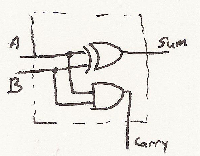
\includegraphics{ha.png} \hspace{.2in} 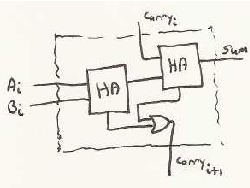
\includegraphics{fa.png}
\end{center}
\end{figure}

\section{Other notes}

Integer numbers larger than the word size of the computer can be handled by chaining.  Two special assembly commands are often available to aid in chaining: addc, subb.   Normally when you add the first carry in is zero, but for blocks of bits after the first block, the lower block might need to carry up.  Addc uses the carry bit as $c_{in}$ rather than assuming $c_{in}=0$.

Two different signals are used to warn that the integer result might not be valid\footnote{Overflow and carry are two of the typical condition codes.  It is possible for a condition code to be set but the result is still valid.  For instance carry could be set and overflow could be unset after an operation with 2's complement numbers.  In this case the number is still valid since overflow is the signal for 2's complement.} : carry (c) and overflow (v).  Carry is used for unsigned integers, and overflow is used for two's complement.  Since both carry and overflow bits are both calculated at the same time\footnote{On some machines every arithmetic operation generates the condition codes, on other machines, like the SPARC, the condition codes are set only when special versions of the arithmetic commands that end in \emph{cc} are used.} it is important to know what they mean, when they are relevant, and how they are calculated.

Overflow set if last two carries are different.



\section{Signed Int}

Addition
\begin{itemize}
    \item if signs are same then add two $n-1$ digit numbers and keep sign
    \item else flip sign of second term and subtract (subtracting with same signs).
\end{itemize}

\noindent
Subtraction ($S_1-S_2$)
\begin{itemize}
    \item if $S_1 \ge S_2 \ge 0$ or $S_1 \le S_2 < 0$ then preserve sign and subtract absolute magnitudes,
    \item if $S_2 > S_1 \ge 0$ or $S_2 < S_1 < 0$ then flip sign and subtract absolute magnitudes reversed,
    \item else flip sign of second term and add (adding with same signs).
\end{itemize}

\section{2's Comp}

For addition you just add the numbers normally with $c_{in}=0$(no special cases).

For subtraction you take the 1's complement of the second number and add with $c_{in}=1$(no special cases, note 1's complement +1 is 2's complement).

\section{Excess}

For addition, you need to carry extra bits while calculating, because you have to subtract the excess number after adding.  This is needed because the excess was in each of the numbers added, so an extra excess is present which must be removed.

For subtraction, the excess gets removed in the process so it must be added back in after subtraction.  Note the subtraction can result in an intermediate negative number, so extra bits are needed during calculation. 